\PassOptionsToPackage{unicode=true}{hyperref} % options for packages loaded elsewhere
\PassOptionsToPackage{hyphens}{url}
%
\documentclass[]{article}
\usepackage{lmodern}
\usepackage{amssymb,amsmath}
\usepackage{ifxetex,ifluatex}
\usepackage{fixltx2e} % provides \textsubscript
\ifnum 0\ifxetex 1\fi\ifluatex 1\fi=0 % if pdftex
  \usepackage[T1]{fontenc}
  \usepackage[utf8]{inputenc}
  \usepackage{textcomp} % provides euro and other symbols
\else % if luatex or xelatex
  \usepackage{unicode-math}
  \defaultfontfeatures{Ligatures=TeX,Scale=MatchLowercase}
\fi
% use upquote if available, for straight quotes in verbatim environments
\IfFileExists{upquote.sty}{\usepackage{upquote}}{}
% use microtype if available
\IfFileExists{microtype.sty}{%
\usepackage[]{microtype}
\UseMicrotypeSet[protrusion]{basicmath} % disable protrusion for tt fonts
}{}
\IfFileExists{parskip.sty}{%
\usepackage{parskip}
}{% else
\setlength{\parindent}{0pt}
\setlength{\parskip}{6pt plus 2pt minus 1pt}
}
\usepackage{hyperref}
\hypersetup{
            pdftitle={Assignment 8: Time Series Analysis},
            pdfauthor={Rachel Gonsenhauser},
            pdfborder={0 0 0},
            breaklinks=true}
\urlstyle{same}  % don't use monospace font for urls
\usepackage[margin=2.54cm]{geometry}
\usepackage{color}
\usepackage{fancyvrb}
\newcommand{\VerbBar}{|}
\newcommand{\VERB}{\Verb[commandchars=\\\{\}]}
\DefineVerbatimEnvironment{Highlighting}{Verbatim}{commandchars=\\\{\}}
% Add ',fontsize=\small' for more characters per line
\usepackage{framed}
\definecolor{shadecolor}{RGB}{248,248,248}
\newenvironment{Shaded}{\begin{snugshade}}{\end{snugshade}}
\newcommand{\AlertTok}[1]{\textcolor[rgb]{0.94,0.16,0.16}{#1}}
\newcommand{\AnnotationTok}[1]{\textcolor[rgb]{0.56,0.35,0.01}{\textbf{\textit{#1}}}}
\newcommand{\AttributeTok}[1]{\textcolor[rgb]{0.77,0.63,0.00}{#1}}
\newcommand{\BaseNTok}[1]{\textcolor[rgb]{0.00,0.00,0.81}{#1}}
\newcommand{\BuiltInTok}[1]{#1}
\newcommand{\CharTok}[1]{\textcolor[rgb]{0.31,0.60,0.02}{#1}}
\newcommand{\CommentTok}[1]{\textcolor[rgb]{0.56,0.35,0.01}{\textit{#1}}}
\newcommand{\CommentVarTok}[1]{\textcolor[rgb]{0.56,0.35,0.01}{\textbf{\textit{#1}}}}
\newcommand{\ConstantTok}[1]{\textcolor[rgb]{0.00,0.00,0.00}{#1}}
\newcommand{\ControlFlowTok}[1]{\textcolor[rgb]{0.13,0.29,0.53}{\textbf{#1}}}
\newcommand{\DataTypeTok}[1]{\textcolor[rgb]{0.13,0.29,0.53}{#1}}
\newcommand{\DecValTok}[1]{\textcolor[rgb]{0.00,0.00,0.81}{#1}}
\newcommand{\DocumentationTok}[1]{\textcolor[rgb]{0.56,0.35,0.01}{\textbf{\textit{#1}}}}
\newcommand{\ErrorTok}[1]{\textcolor[rgb]{0.64,0.00,0.00}{\textbf{#1}}}
\newcommand{\ExtensionTok}[1]{#1}
\newcommand{\FloatTok}[1]{\textcolor[rgb]{0.00,0.00,0.81}{#1}}
\newcommand{\FunctionTok}[1]{\textcolor[rgb]{0.00,0.00,0.00}{#1}}
\newcommand{\ImportTok}[1]{#1}
\newcommand{\InformationTok}[1]{\textcolor[rgb]{0.56,0.35,0.01}{\textbf{\textit{#1}}}}
\newcommand{\KeywordTok}[1]{\textcolor[rgb]{0.13,0.29,0.53}{\textbf{#1}}}
\newcommand{\NormalTok}[1]{#1}
\newcommand{\OperatorTok}[1]{\textcolor[rgb]{0.81,0.36,0.00}{\textbf{#1}}}
\newcommand{\OtherTok}[1]{\textcolor[rgb]{0.56,0.35,0.01}{#1}}
\newcommand{\PreprocessorTok}[1]{\textcolor[rgb]{0.56,0.35,0.01}{\textit{#1}}}
\newcommand{\RegionMarkerTok}[1]{#1}
\newcommand{\SpecialCharTok}[1]{\textcolor[rgb]{0.00,0.00,0.00}{#1}}
\newcommand{\SpecialStringTok}[1]{\textcolor[rgb]{0.31,0.60,0.02}{#1}}
\newcommand{\StringTok}[1]{\textcolor[rgb]{0.31,0.60,0.02}{#1}}
\newcommand{\VariableTok}[1]{\textcolor[rgb]{0.00,0.00,0.00}{#1}}
\newcommand{\VerbatimStringTok}[1]{\textcolor[rgb]{0.31,0.60,0.02}{#1}}
\newcommand{\WarningTok}[1]{\textcolor[rgb]{0.56,0.35,0.01}{\textbf{\textit{#1}}}}
\usepackage{graphicx,grffile}
\makeatletter
\def\maxwidth{\ifdim\Gin@nat@width>\linewidth\linewidth\else\Gin@nat@width\fi}
\def\maxheight{\ifdim\Gin@nat@height>\textheight\textheight\else\Gin@nat@height\fi}
\makeatother
% Scale images if necessary, so that they will not overflow the page
% margins by default, and it is still possible to overwrite the defaults
% using explicit options in \includegraphics[width, height, ...]{}
\setkeys{Gin}{width=\maxwidth,height=\maxheight,keepaspectratio}
\setlength{\emergencystretch}{3em}  % prevent overfull lines
\providecommand{\tightlist}{%
  \setlength{\itemsep}{0pt}\setlength{\parskip}{0pt}}
\setcounter{secnumdepth}{0}
% Redefines (sub)paragraphs to behave more like sections
\ifx\paragraph\undefined\else
\let\oldparagraph\paragraph
\renewcommand{\paragraph}[1]{\oldparagraph{#1}\mbox{}}
\fi
\ifx\subparagraph\undefined\else
\let\oldsubparagraph\subparagraph
\renewcommand{\subparagraph}[1]{\oldsubparagraph{#1}\mbox{}}
\fi

% set default figure placement to htbp
\makeatletter
\def\fps@figure{htbp}
\makeatother


\title{Assignment 8: Time Series Analysis}
\author{Rachel Gonsenhauser}
\date{}

\begin{document}
\maketitle

\hypertarget{overview}{%
\subsection{OVERVIEW}\label{overview}}

This exercise accompanies the lessons in Environmental Data Analytics on
time series analysis.

\hypertarget{directions}{%
\subsection{Directions}\label{directions}}

\begin{enumerate}
\def\labelenumi{\arabic{enumi}.}
\tightlist
\item
  Change ``Student Name'' on line 3 (above) with your name.
\item
  Work through the steps, \textbf{creating code and output} that fulfill
  each instruction.
\item
  Be sure to \textbf{answer the questions} in this assignment document.
\item
  When you have completed the assignment, \textbf{Knit} the text and
  code into a single PDF file.
\item
  After Knitting, submit the completed exercise (PDF file) to the
  dropbox in Sakai. Add your last name into the file name (e.g.,
  ``Salk\_A06\_GLMs\_Week1.Rmd'') prior to submission.
\end{enumerate}

The completed exercise is due on Tuesday, March 3 at 1:00 pm.

\hypertarget{set-up}{%
\subsection{Set up}\label{set-up}}

\begin{enumerate}
\def\labelenumi{\arabic{enumi}.}
\tightlist
\item
  Set up your session:
\end{enumerate}

\begin{itemize}
\tightlist
\item
  Check your working directory
\item
  Load the tidyverse, lubridate, zoo, and trend packages
\item
  Set your ggplot theme
\item
  Import the ten datasets from the Ozone\_TimeSeries folder in the Raw
  data folder. These contain ozone concentrations at Garinger High
  School in North Carolina from 2010-2019 (the EPA air database only
  allows downloads for one year at a time). Call these
  GaringerOzone201*, with the star filled in with the appropriate year
  in each of ten cases.
\end{itemize}

\begin{Shaded}
\begin{Highlighting}[]
\KeywordTok{getwd}\NormalTok{()}
\end{Highlighting}
\end{Shaded}

\begin{verbatim}
## [1] "/Users/rachelgonsenhauser/Documents/Environmental_Data_Analytics_2020"
\end{verbatim}

\begin{Shaded}
\begin{Highlighting}[]
\KeywordTok{library}\NormalTok{(tidyverse)}
\KeywordTok{library}\NormalTok{(lubridate)}
\KeywordTok{library}\NormalTok{(zoo)}
\KeywordTok{library}\NormalTok{(trend)}

\NormalTok{mytheme <-}\StringTok{ }\KeywordTok{theme_classic}\NormalTok{(}\DataTypeTok{base_size =} \DecValTok{12}\NormalTok{) }\OperatorTok{+}
\StringTok{  }\KeywordTok{theme}\NormalTok{(}\DataTypeTok{axis.text =} \KeywordTok{element_text}\NormalTok{(}\DataTypeTok{color =} \StringTok{"black"}\NormalTok{),}
        \DataTypeTok{legend.position =} \StringTok{"bottom"}\NormalTok{)}
\KeywordTok{theme_set}\NormalTok{(mytheme)}

\NormalTok{GaringerOzone2010 <-}\StringTok{ }\KeywordTok{read.csv}\NormalTok{(}\StringTok{"./Data/Raw/Ozone_TimeSeries/EPAair_O3_GaringerNC2010_raw.csv"}\NormalTok{)}
\NormalTok{GaringerOzone2011 <-}\StringTok{ }\KeywordTok{read.csv}\NormalTok{(}\StringTok{"./Data/Raw/Ozone_TimeSeries/EPAair_O3_GaringerNC2011_raw.csv"}\NormalTok{)}
\NormalTok{GaringerOzone2012 <-}\StringTok{ }\KeywordTok{read.csv}\NormalTok{(}\StringTok{"./Data/Raw/Ozone_TimeSeries/EPAair_O3_GaringerNC2012_raw.csv"}\NormalTok{)}
\NormalTok{GaringerOzone2013 <-}\StringTok{ }\KeywordTok{read.csv}\NormalTok{(}\StringTok{"./Data/Raw/Ozone_TimeSeries/EPAair_O3_GaringerNC2013_raw.csv"}\NormalTok{)}
\NormalTok{GaringerOzone2014 <-}\StringTok{ }\KeywordTok{read.csv}\NormalTok{(}\StringTok{"./Data/Raw/Ozone_TimeSeries/EPAair_O3_GaringerNC2014_raw.csv"}\NormalTok{)}
\NormalTok{GaringerOzone2015 <-}\StringTok{ }\KeywordTok{read.csv}\NormalTok{(}\StringTok{"./Data/Raw/Ozone_TimeSeries/EPAair_O3_GaringerNC2015_raw.csv"}\NormalTok{)}
\NormalTok{GaringerOzone2016 <-}\StringTok{ }\KeywordTok{read.csv}\NormalTok{(}\StringTok{"./Data/Raw/Ozone_TimeSeries/EPAair_O3_GaringerNC2016_raw.csv"}\NormalTok{)}
\NormalTok{GaringerOzone2017 <-}\StringTok{ }\KeywordTok{read.csv}\NormalTok{(}\StringTok{"./Data/Raw/Ozone_TimeSeries/EPAair_O3_GaringerNC2017_raw.csv"}\NormalTok{)}
\NormalTok{GaringerOzone2018 <-}\StringTok{ }\KeywordTok{read.csv}\NormalTok{(}\StringTok{"./Data/Raw/Ozone_TimeSeries/EPAair_O3_GaringerNC2018_raw.csv"}\NormalTok{)}
\NormalTok{GaringerOzone2019 <-}\StringTok{ }\KeywordTok{read.csv}\NormalTok{(}\StringTok{"./Data/Raw/Ozone_TimeSeries/EPAair_O3_GaringerNC2019_raw.csv"}\NormalTok{)}
\end{Highlighting}
\end{Shaded}

\hypertarget{wrangle}{%
\subsection{Wrangle}\label{wrangle}}

\begin{enumerate}
\def\labelenumi{\arabic{enumi}.}
\setcounter{enumi}{1}
\item
  Combine your ten datasets into one dataset called GaringerOzone. Think
  about whether you should use a join or a row bind.
\item
  Set your date column as a date class.
\item
  Wrangle your dataset so that it only contains the columns Date,
  Daily.Max.8.hour.Ozone.Concentration, and DAILY\_AQI\_VALUE.
\item
  Notice there are a few days in each year that are missing ozone
  concentrations. We want to generate a daily dataset, so we will need
  to fill in any missing days with NA. Create a new data frame that
  contains a sequence of dates from 2010-01-01 to 2019-12-13 (hint:
  \texttt{as.data.frame(seq())}). Call this new data frame Days. Rename
  the column name in Days to ``Date''.
\item
  Use a \texttt{left\_join} to comine the data frames. Specify the
  correct order of data frames within this function so that the final
  dimensions are 3652 rows and 3 columns. Call your combined data frame
  GaringerOzone.
\end{enumerate}

\begin{Shaded}
\begin{Highlighting}[]
\CommentTok{# 2 }
\NormalTok{GaringerOzone <-}\StringTok{ }\KeywordTok{rbind}\NormalTok{(GaringerOzone2010, GaringerOzone2011, GaringerOzone2012, GaringerOzone2013, GaringerOzone2014, GaringerOzone2015, GaringerOzone2016, GaringerOzone2017, GaringerOzone2018, GaringerOzone2019)}

\CommentTok{# 3}
\NormalTok{GaringerOzone}\OperatorTok{$}\NormalTok{Date <-}\StringTok{ }\KeywordTok{as.Date}\NormalTok{(GaringerOzone}\OperatorTok{$}\NormalTok{Date, }\DataTypeTok{format =} \StringTok{"%m/%d/%Y"}\NormalTok{)}
\KeywordTok{class}\NormalTok{(GaringerOzone}\OperatorTok{$}\NormalTok{Date)}
\end{Highlighting}
\end{Shaded}

\begin{verbatim}
## [1] "Date"
\end{verbatim}

\begin{Shaded}
\begin{Highlighting}[]
\CommentTok{# 4}
\NormalTok{GaringerOzone.wrangled <-}\StringTok{ }
\StringTok{  }\NormalTok{GaringerOzone }\OperatorTok
\StringTok{  }\KeywordTok{select}\NormalTok{(Date, Daily.Max.}\FloatTok{8.}\NormalTok{hour.Ozone.Concentration, DAILY_AQI_VALUE)}

\CommentTok{# 5}
\NormalTok{Days <-}
\StringTok{  }\KeywordTok{as.data.frame}\NormalTok{(}\KeywordTok{seq}\NormalTok{(}\KeywordTok{as.Date}\NormalTok{(}\StringTok{'2010-01-01'}\NormalTok{),}
                     \KeywordTok{as.Date}\NormalTok{(}\StringTok{'2019-12-31'}\NormalTok{), }\DataTypeTok{by =} \StringTok{'days'}\NormalTok{), }\DataTypeTok{times =}\NormalTok{ num_repeat)}
\KeywordTok{colnames}\NormalTok{(Days) <-}\StringTok{ }\KeywordTok{c}\NormalTok{(}\StringTok{"Date"}\NormalTok{)}

\CommentTok{# 6}
\NormalTok{GaringerOzone <-}\StringTok{ }\KeywordTok{left_join}\NormalTok{(Days,}
\NormalTok{                           GaringerOzone.wrangled)}
\end{Highlighting}
\end{Shaded}

\begin{verbatim}
## Joining, by = "Date"
\end{verbatim}

\hypertarget{visualize}{%
\subsection{Visualize}\label{visualize}}

\begin{enumerate}
\def\labelenumi{\arabic{enumi}.}
\setcounter{enumi}{6}
\tightlist
\item
  Create a ggplot depicting ozone concentrations over time. In this
  case, we will plot actual concentrations in ppm, not AQI values.
  Format your axes accordingly.
\end{enumerate}

\begin{Shaded}
\begin{Highlighting}[]
\CommentTok{#library(RColorBrewer)}

\NormalTok{GaringerOzonePlot <-}\StringTok{ }
\StringTok{  }\KeywordTok{ggplot}\NormalTok{(GaringerOzone, }\KeywordTok{aes}\NormalTok{(}\DataTypeTok{x =}\NormalTok{ Date, }\DataTypeTok{y =}\NormalTok{ Daily.Max.}\FloatTok{8.}\NormalTok{hour.Ozone.Concentration, }\DataTypeTok{alpha =} \FloatTok{0.5}\NormalTok{)) }\OperatorTok{+}
\StringTok{  }\KeywordTok{geom_point}\NormalTok{(}\DataTypeTok{color =} \StringTok{"dark green"}\NormalTok{) }\OperatorTok{+}
\StringTok{  }\KeywordTok{labs}\NormalTok{(}\DataTypeTok{x =} \StringTok{"Date"}\NormalTok{, }\DataTypeTok{y =} \StringTok{"Ozone concentration (ppm)"}\NormalTok{) }\OperatorTok{+}
\StringTok{  }\KeywordTok{scale_color_brewer}\NormalTok{(}\DataTypeTok{palette =} \StringTok{"Paired"}\NormalTok{) }
\KeywordTok{print}\NormalTok{(GaringerOzonePlot)}
\end{Highlighting}
\end{Shaded}

\begin{verbatim}
## Warning: Removed 63 rows containing missing values (geom_point).
\end{verbatim}

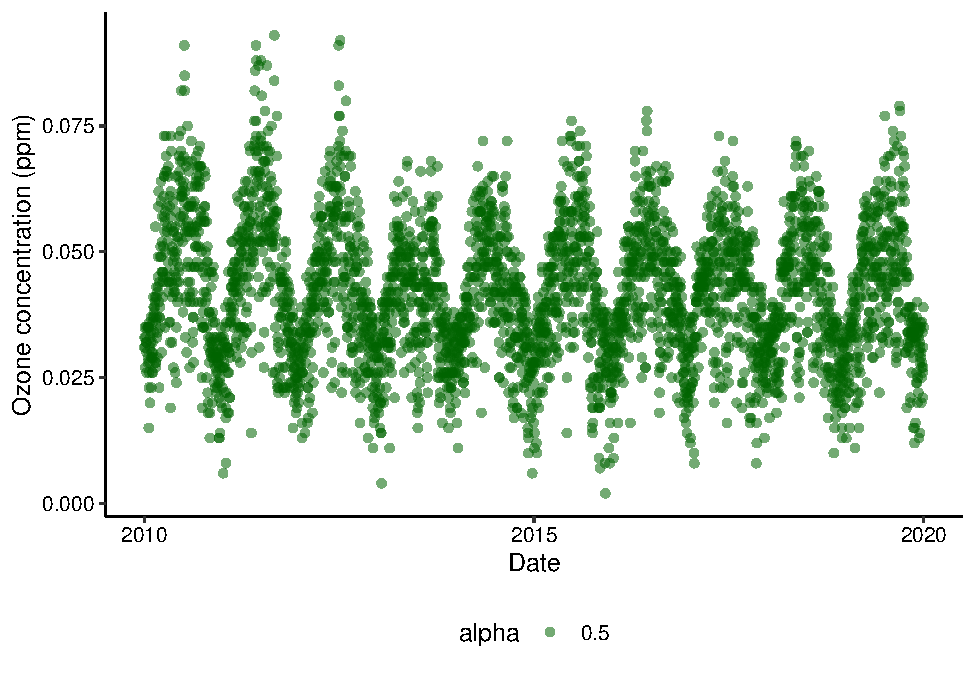
\includegraphics{A08_TimeSeries_files/figure-latex/unnamed-chunk-3-1.pdf}

\hypertarget{time-series-analysis}{%
\subsection{Time Series Analysis}\label{time-series-analysis}}

Study question: Have ozone concentrations changed over the 2010s at this
station?

\begin{enumerate}
\def\labelenumi{\arabic{enumi}.}
\setcounter{enumi}{7}
\tightlist
\item
  Use a linear interpolation to fill in missing daily data for ozone
  concentration. Why didn't we use a piecewise constant or spline
  interpolation?
\end{enumerate}

\begin{quote}
Answer: In this case, linear interpolation is the most appropriate
method due to temporal autocorrelation. Missing ozone concentrations are
likely to be close to those on the preceding and follow days, so using
linear interpolation is logical as this method fills data gaps with
values that fall between the previous and next measurement. The
piecewise constant method is inappropriate as missing ozone
concentrations are not necessarily equal to measurements made nearest to
that date. Additionally, there are not large chunks of missing data in
the dataset, so the spine interpolation method also seems inappropriate
in this case.
\end{quote}

\begin{enumerate}
\def\labelenumi{\arabic{enumi}.}
\setcounter{enumi}{8}
\item
  Create a new data frame called GaringerOzone.monthly that contains
  aggregated data: mean ozone concentrations for each month. In your
  pipe, you will need to first add columns for year and month to form
  the groupings. In a separate line of code, create a new Date column
  with each month-year combination being set as the first day of the
  month (this is for graphing purposes only)
\item
  Generate a time series called GaringerOzone.monthly.ts, with a monthly
  frequency that specifies the correct start and end dates.
\item
  Run a time series analysis. In this case the seasonal Mann-Kendall is
  most appropriate; why is this?
\end{enumerate}

\begin{quote}
Answer: The seasonal Mann-Kendall is the most appropriate time series
analysis to run in this case because it is the only test that assumes
seasonality. Our plot above seems to exhibit a seasonal trend to the
data, so the seasonal Mann-Kendall analysis is the most fitting.
\end{quote}

\begin{enumerate}
\def\labelenumi{\arabic{enumi}.}
\setcounter{enumi}{11}
\item
  To figure out the slope of the trend, run the function
  \texttt{sea.sens.slope} on the time series dataset.
\item
  Create a plot depicting mean monthly ozone concentrations over time,
  with both a geom\_point and a geom\_line layer. No need to add a line
  for the seasonal Sen's slope; this is difficult to apply to a graph
  with time as the x axis. Edit your axis labels accordingly.
\end{enumerate}

\begin{Shaded}
\begin{Highlighting}[]
\CommentTok{# 8}
\NormalTok{GaringerOzone}\OperatorTok{$}\NormalTok{Daily.Max.}\FloatTok{8.}\NormalTok{hour.Ozone.Concentration <-}\StringTok{ }\KeywordTok{na.approx}\NormalTok{(GaringerOzone}\OperatorTok{$}\NormalTok{Daily.Max.}\FloatTok{8.}\NormalTok{hour.Ozone.Concentration)}

\CommentTok{# 9}
\NormalTok{GaringerOzone.monthly  <-}\StringTok{ }\NormalTok{GaringerOzone }\OperatorTok
\StringTok{  }\KeywordTok{mutate}\NormalTok{(}\DataTypeTok{Year =} \KeywordTok{year}\NormalTok{(Date),}
\DataTypeTok{Month =} \KeywordTok{month}\NormalTok{(Date)) }\OperatorTok
\StringTok{  }\KeywordTok{group_by}\NormalTok{(Year, Month) }\OperatorTok
\StringTok{  }\KeywordTok{summarise}\NormalTok{(}\DataTypeTok{Daily.Max.8.hour.Ozone.Concentration =} \KeywordTok{mean}\NormalTok{(Daily.Max.}\FloatTok{8.}\NormalTok{hour.Ozone.Concentration))}
  
\NormalTok{GaringerOzone.monthly}\OperatorTok{$}\NormalTok{Date <-}\StringTok{ }\KeywordTok{as.Date}\NormalTok{(}\KeywordTok{paste}\NormalTok{(GaringerOzone.monthly}\OperatorTok{$}\NormalTok{Year, }
\NormalTok{                                                GaringerOzone.monthly}\OperatorTok{$}\NormalTok{Month, }\DecValTok{1}\NormalTok{, }\DataTypeTok{sep=}\StringTok{"-"}\NormalTok{),}
                                      \DataTypeTok{format =} \StringTok{"%Y-%m-%d"}\NormalTok{)}

\CommentTok{# 10}
\NormalTok{GaringerOzone.monthly.ts <-}
\StringTok{  }\KeywordTok{ts}\NormalTok{(GaringerOzone.monthly}\OperatorTok{$}\NormalTok{Daily.Max.}\FloatTok{8.}\NormalTok{hour.Ozone.Concentration, }\DataTypeTok{frequency =} \DecValTok{12}\NormalTok{, }
                        \DataTypeTok{start =} \KeywordTok{c}\NormalTok{(}\DecValTok{2010}\NormalTok{, }\DecValTok{01}\NormalTok{, }\DecValTok{01}\NormalTok{), }\DataTypeTok{end =} \KeywordTok{c}\NormalTok{(}\DecValTok{2019}\NormalTok{, }\DecValTok{12}\NormalTok{, }\DecValTok{31}\NormalTok{))}

\CommentTok{# 11}
\NormalTok{GaringerOzone.trend <-}\StringTok{ }\KeywordTok{smk.test}\NormalTok{(GaringerOzone.monthly.ts)}
\NormalTok{GaringerOzone.trend}
\end{Highlighting}
\end{Shaded}

\begin{verbatim}
## 
##  Seasonal Mann-Kendall trend test (Hirsch-Slack test)
## 
## data:  GaringerOzone.monthly.ts
## z = -1.963, p-value = 0.04965
## alternative hypothesis: true S is not equal to 0
## sample estimates:
##    S varS 
##  -77 1499
\end{verbatim}

\begin{Shaded}
\begin{Highlighting}[]
\KeywordTok{summary}\NormalTok{(GaringerOzone.trend)}
\end{Highlighting}
\end{Shaded}

\begin{verbatim}
## 
##  Seasonal Mann-Kendall trend test (Hirsch-Slack test)
## 
## data: GaringerOzone.monthly.ts
## alternative hypothesis: two.sided
## 
## Statistics for individual seasons
## 
## H0
##                      S varS    tau      z Pr(>|z|)  
## Season 1:   S = 0   15  125  0.333  1.252  0.21050  
## Season 2:   S = 0   -1  125 -0.022  0.000  1.00000  
## Season 3:   S = 0   -4  124 -0.090 -0.269  0.78762  
## Season 4:   S = 0  -17  125 -0.378 -1.431  0.15241  
## Season 5:   S = 0  -15  125 -0.333 -1.252  0.21050  
## Season 6:   S = 0  -17  125 -0.378 -1.431  0.15241  
## Season 7:   S = 0  -11  125 -0.244 -0.894  0.37109  
## Season 8:   S = 0   -7  125 -0.156 -0.537  0.59151  
## Season 9:   S = 0   -5  125 -0.111 -0.358  0.72051  
## Season 10:   S = 0 -13  125 -0.289 -1.073  0.28313  
## Season 11:   S = 0 -13  125 -0.289 -1.073  0.28313  
## Season 12:   S = 0  11  125  0.244  0.894  0.37109  
## ---
## Signif. codes:  0 '***' 0.001 '**' 0.01 '*' 0.05 '.' 0.1 ' ' 1
\end{verbatim}

\begin{Shaded}
\begin{Highlighting}[]
\CommentTok{# 12}
\KeywordTok{sea.sens.slope}\NormalTok{(GaringerOzone.monthly.ts)}
\end{Highlighting}
\end{Shaded}

\begin{verbatim}
## [1] -0.0002044163
\end{verbatim}

\begin{Shaded}
\begin{Highlighting}[]
\CommentTok{# 13}

\NormalTok{GaringerOzonePlot.monthly <-}
\StringTok{  }\KeywordTok{ggplot}\NormalTok{(GaringerOzone.monthly, }
         \KeywordTok{aes}\NormalTok{(}\DataTypeTok{x =}\NormalTok{ Date, }\DataTypeTok{y =}\NormalTok{ Daily.Max.}\FloatTok{8.}\NormalTok{hour.Ozone.Concentration)) }\OperatorTok{+}
\StringTok{   }\KeywordTok{geom_point}\NormalTok{(}\DataTypeTok{color =} \StringTok{"cadet blue"}\NormalTok{) }\OperatorTok{+}
\StringTok{  }\KeywordTok{geom_line}\NormalTok{(}\DataTypeTok{color =} \StringTok{"cadet blue"}\NormalTok{) }\OperatorTok{+}
\StringTok{  }\KeywordTok{labs}\NormalTok{(}\DataTypeTok{x =} \StringTok{"Date"}\NormalTok{, }\DataTypeTok{y =} \StringTok{"Ozone concentration (ppm)"}\NormalTok{) }
\KeywordTok{print}\NormalTok{(GaringerOzonePlot.monthly)}
\end{Highlighting}
\end{Shaded}

\includegraphics{A08_TimeSeries_files/figure-latex/unnamed-chunk-4-1.pdf}

\begin{enumerate}
\def\labelenumi{\arabic{enumi}.}
\setcounter{enumi}{13}
\tightlist
\item
  To accompany your graph, summarize your results in context of the
  research question. Include output from the statistical test in
  parentheses at the end of your sentence. Feel free to use multiple
  sentences in your interpretation.
\end{enumerate}

\begin{quote}
Answer: There is a significant monotonic trend in ozone concentration
data at Garinger High School over the period of 2010-2019 (seasonal
Mann-Kendall: z=-1.963, p=0.04965). The slope of this trend indicates
that ozone concentrations are slightly decreasing over the period of
2010-2019 at Garinger High School (Sen's Slope=-0.000207152). We did not
detect any seasonal trends across individual months in the dataset.
\end{quote}

\end{document}
